\documentclass[border=10pt]{standalone}

\usepackage{tikz}
\usepackage{tikzsymbols}
\usetikzlibrary{calc,patterns,shapes.geometric}

\def\centerarc[#1](#2)(#3:#4:#5){\draw[#1] ($(#2)+({#5*cos(#3)},{#5*sin(#3)})$) arc (#3:#4:#5);}

\begin{document}
	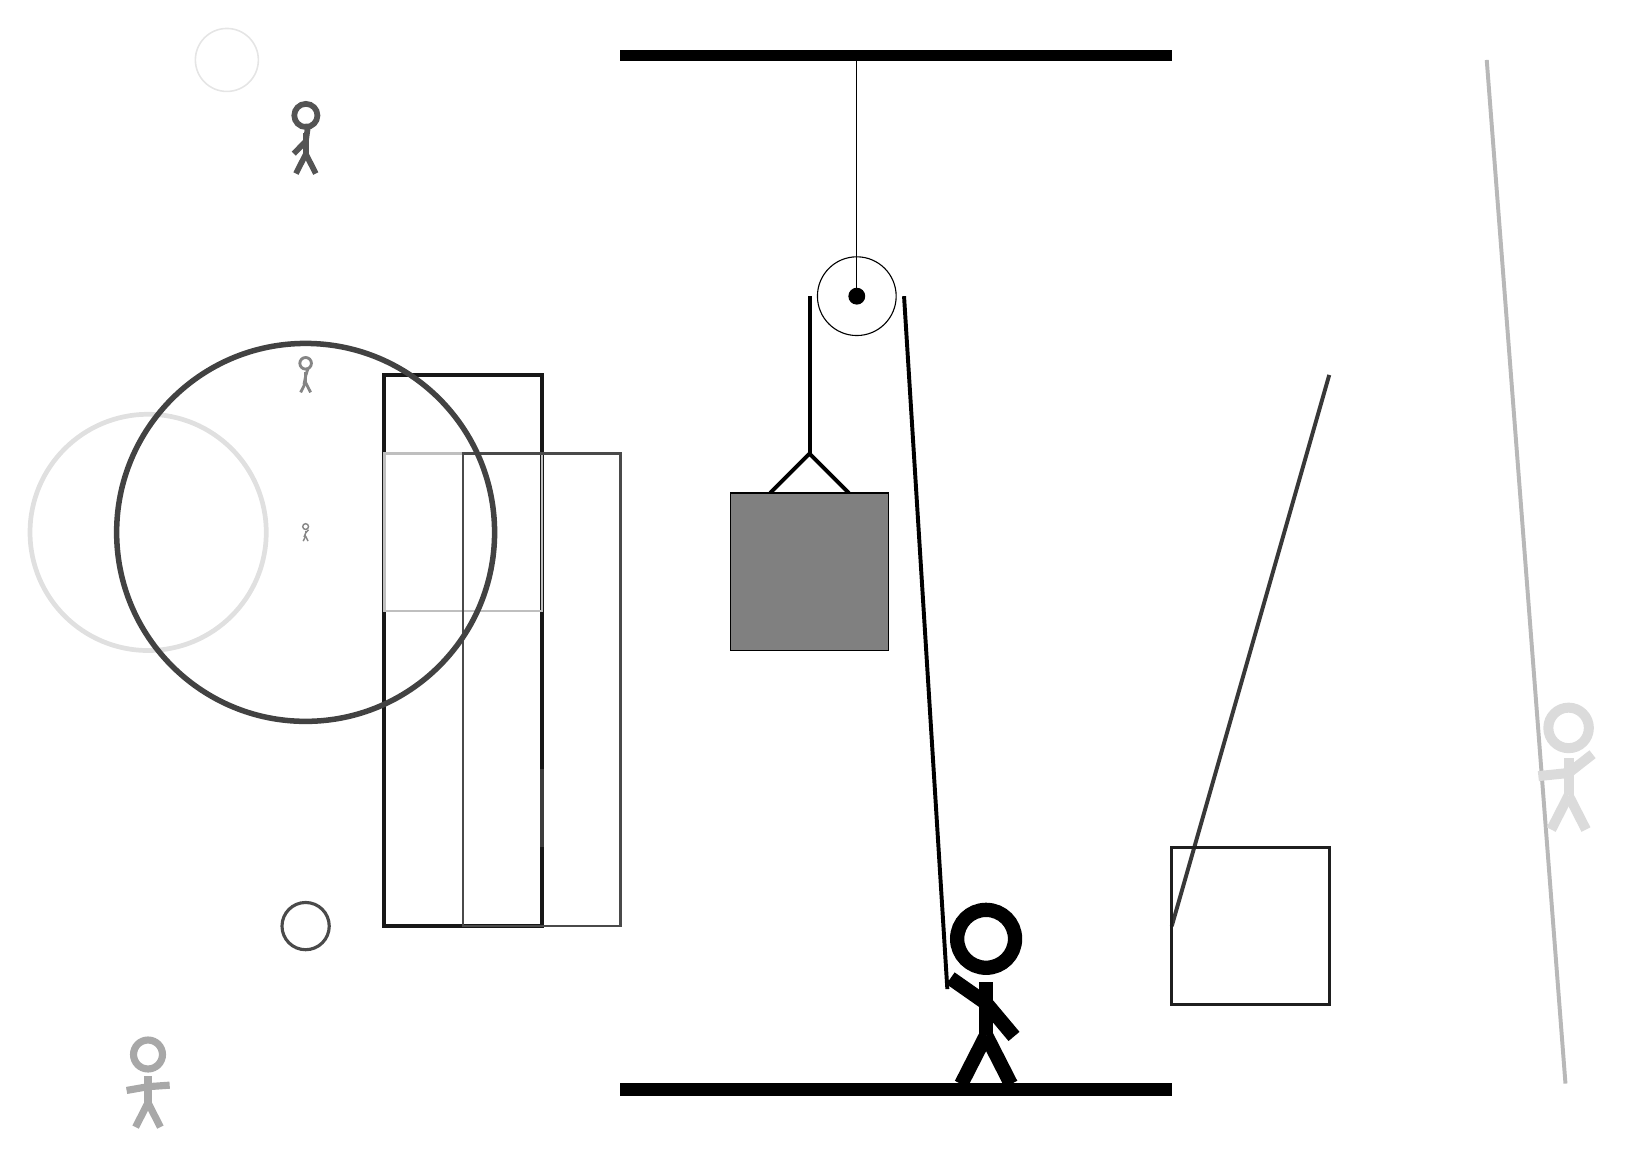
\begin{tikzpicture}
		%%%%% START %%%%%
		
		\draw[fill=black] (-2, 10) rectangle (5, 10.125);
		
		\draw (1, 7) circle (0.5);
		\draw[fill=black] (1, 7) circle (0.1);
		\draw (1, 10) -- (1, 7);
		
		\draw[line width=0.5mm] (-0.1, 4.5) -- (0.4, 5.0) -- (0.9, 4.5);
		\draw[fill=black!50] (-0.6, 4.5) rectangle (1.4, 2.5);
		
		\draw[line width=0.5mm] (0.4, 7) -- (0.4, 5.0);
		\centerarc[line width=0.5mm](1, 7)(0:180:0.6);
		\draw[line width=0.5mm](1.6, 7) -- (2.15, -1.8);
		
		\node at (2.6, -1.9) {\Strichmaxerl[10][-35][-50]};
		
		\node[line width=0.5mm, color=black!48] at (-6, 6) {\Strichmaxerl[2][79][73]};
		
		\draw [line width=0.4mm, color=black!71](-6, -1) circle (0.3);
		\draw[line width=0.5mm, color=black!91] (-3, 6) rectangle (-5, -1);
		\draw[line width=0.3mm, color=black!25] (-3, 3) rectangle (-5, 5);
		\draw[line width=0.5mm, color=black!28](9, 10) -- (10, -3);
		
		\node[line width=0.3mm, color=black!14] at (10, 1) {\Strichmaxerl[7][6][38]};
		
		\draw[line width=0.5mm, color=black!78](5, -1) -- (7, 6);
		\node[line width=0.6mm, color=black!67] at (-6, 9) {\Strichmaxerl[4][46][82]};
		\draw[line width=0.3mm, color=black!71] (-2, -1) rectangle (-4, 5);
		\draw [line width=0.6mm, color=black!12](-8, 4) circle (1.5);
		
		\node[line width=0.5mm, color=black!47] at (-6, 4) {\Strichmaxerl[1][68][49]};
		
		\draw[line width=0.5mm, color=black!76](-3, 0) -- (-3, 1);
		\draw[line width=0.4mm, color=black!88] (5, -2) rectangle (7, 0);
		\draw [line width=0.2mm, color=black!10](-7, 10) circle (0.4);
		\node[line width=0.4mm, color=black!34] at (-8, -3) {\Strichmaxerl[5][10][4]};
		\draw [line width=0.7mm, color=black!74](-6, 4) circle (2.4);
		
		
		\draw[fill=black] (-2, -3) rectangle (5, -3.15);
		
		%%%%% END %%%%%
	\end{tikzpicture}
\end{document}